\documentclass{minimal}
\usepackage{amsmath}
\usepackage{tikz}
\usetikzlibrary{arrows.meta}

\begin{document}
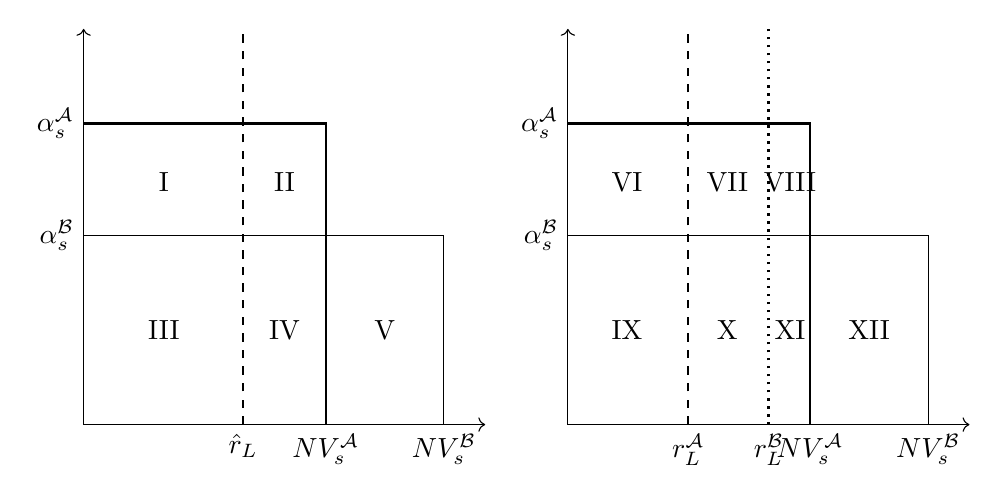
\begin{tikzpicture}[scale=1.5]

% Common levels
\def\alphaA{2.55}
\def\alphaB{1.60}

% Left Plot
\draw[->] (0,0) -- (3.4,0);
\draw[->] (0,0) -- (0,3.35);

% Solid phase boundaries
\draw[line width=0.9pt] (0,\alphaA) -- (2.05,\alphaA) -- (2.05,0);
\draw (0,\alphaB) -- (3.05,\alphaB) -- (3.05,0);

% Interest-rate separator
\draw[dashed,line width=0.8pt] (1.35,0) -- (1.35,3.35);

\node at (0.68,2.05) {I};
\node at (1.70,2.05) {II};
\node at (0.68,0.80) {III};
\node at (1.70,0.80) {IV};
\node at (2.55,0.80) {V};

\node[below] at (1.35,0) {$\hat{r}_L$};
\node[below] at (2.05,0) {$NV_s^{\mathcal{A}}$};
\node[below] at (3.05,0) {$NV_s^{\mathcal{B}}$};
\node[left] at (0,\alphaA) {$\alpha_s^{\mathcal{A}}$};
\node[left] at (0,\alphaB) {$\alpha_s^{\mathcal{B}}$};

% Right Plot
\begin{scope}[xshift=4.1cm]
\draw[->] (0,0) -- (3.4,0);
\draw[->] (0,0) -- (0,3.35);

% Solid phase boundaries
\draw[line width=0.9pt] (0,\alphaA) -- (2.05,\alphaA) -- (2.05,0);
\draw (0,\alphaB) -- (3.05,\alphaB) -- (3.05,0);

% Interest-rate separators
\draw[dashed,line width=0.8pt] (1.02,0) -- (1.02,3.35);
\draw[dotted,line width=0.9pt] (1.70,0) -- (1.70,3.35);

\node at (0.50,2.05) {VI};
\node at (1.35,2.05) {VII};
\node at (1.88,2.05) {VIII};
\node at (0.50,0.80) {IX};
\node at (1.35,0.80) {X};
\node at (1.88,0.80) {XI};
\node at (2.55,0.80) {XII};

\node[below] at (1.02,0) {$r_L^{\mathcal{A}}$};
\node[below] at (1.70,0) {$r_L^{\mathcal{B}}$};
\node[below] at (2.05,0) {$NV_s^{\mathcal{A}}$};
\node[below] at (3.05,0) {$NV_s^{\mathcal{B}}$};
\node[left] at (0,\alphaA) {$\alpha_s^{\mathcal{A}}$};
\node[left] at (0,\alphaB) {$\alpha_s^{\mathcal{B}}$};
\end{scope}

\end{tikzpicture}
\end{document}
